%This is a Tex Version of Math 304 Homework Template
%

\documentclass{amsart}
\setlength{\textheight}{9in}
\setlength{\topmargin}{-0.5in}
\setlength{\textwidth}{7in}
\setlength{\evensidemargin}{-0.25in}
\setlength{\oddsidemargin}{-0.25in}
\usepackage{amsfonts}
\usepackage[T1]{fontenc}
\usepackage{graphicx}             % needed to include these graphics
%\graphicspath{{./Pictures/}}      % only in case you want to keep the pictures in a separate subdirectory; also see the appropriate line below
\usepackage{caption}
\usepackage{subcaption}
\usepackage{float}
\newcounter{temp}
\theoremstyle{definition}
\newtheorem{Thm}{Theorem}
\newtheorem{Prob}{Problem}
\newtheorem*{Def}{Definition}
\newtheorem*{Ans}{Answer}
\newcommand{\dis}{\displaystyle}
\newcommand{\dlim}{\dis\lim}
\newcommand{\dsum}{\dis\sum}
\newcommand{\dint}{\dis\int}
\newcommand{\ddint}{\dint\!\!\dint}
\newcommand{\dddint}{\dint\!\!\dint\!\!\dint}
\newcommand{\dt}{\text{d}t}
\newcommand{\dA}{\text{d}A}
\newcommand{\dV}{\text{d}V}
\newcommand{\dx}{\text{d}x}
\newcommand{\dy}{\text{d}y}
\newcommand{\dz}{\text{d}z}
\newcommand{\dw}{\text{d}w}
\newcommand{\du}{\text{d}u}
\newcommand{\dv}{\text{d}v}
\newcommand{\ds}{\text{d}s}
\newcommand{\dr}{\text{d}r}
\newcommand{\dth}{\text{d}\theta}
\newcommand{\bbR}{\mathbb{R}}
\newcommand{\bbN}{\mathbb{N}}
\newcommand{\bbQ}{\mathbb{Q}}
\newcommand{\bbZ}{\mathbb{Z}}
\newcommand{\bbC}{\mathbb{C}}
\newcommand{\dd}[2]{\dfrac{\text{d}#1}{\text{d}#2}}
\newcommand{\dydx}{\dfrac{\text{d}y}{\text{d}x}}
\renewcommand{\labelenumi}{{\normalfont \arabic{enumi}.}}
\renewcommand{\labelenumii}{{\normalfont \alph{enumii}.}}
\renewcommand{\labelenumiii}{{\normalfont \roman{enumiii}.}}
\font \bggbf cmbx18 scaled \magstep2
\font \bgbf cmbx10 scaled \magstep2

%% 
% Minoo's added packages:
% Extra spacing features,e.g. placing more than one equation in a line and aligning multiple equations in separate lines:
\usepackage{amsmath} 

% "Corresponds to" symbol:
\usepackage{scalerel,stackengine}
\newcommand\equalhat{\mathrel{\stackon[1.5pt]{=}{\stretchto{%
    \scalerel*[\widthof{=}]{\wedge}{\rule{1ex}{3ex}}}{0.5ex}}}}

% Coloring and highlighting the text:
\usepackage{color,soul}

% Header and footer, page numbering, etc:
\usepackage[english]{babel}
\usepackage[utf8]{inputenc}
\usepackage{fancyhdr}
\usepackage{lastpage}
\pagestyle{fancy}
\fancyhf{}
\rhead{\textit{Minoo's Notes}} % right header
\lhead{Signal Processing} % left header
\rfoot{Page \thepage \hspace{1pt} of \pageref{LastPage}} % page number

% Highlighting an equation:
\usepackage{xcolor}
\newcommand{\highlight}[1]{%
  \colorbox{yellow!50}{$\displaystyle#1$}}  
%%

\title {Signal processing}
\begin{document}
\begin{center}
	{\bgbf Signal processing\\ \smallskip
	Fourier Series\\ \smallskip
	Spring 2017\\ \smallskip
	Minoo's practices}
\end{center}
\vspace{1.25cm}

\begin{enumerate}
    \item General formula for Fourier series:
           
           \begin{equation*}
f(x) \approx a_0 + \sum_{n=1}^{N} [a_n \cos (n \frac {2 \pi} {\tau} x) + b_n \sin (n \frac {2 \pi} {\tau} x)]
\end{equation*}
            
            where
            \begin{align*}
            a_0 &= \frac {1}{\tau} \int_{S}^{S+\tau} f(x) \dx \\
            a_n &= \frac {2}{\tau} \int_{S}^{S+\tau} f(x) \cos (n \frac {2 \pi}{\tau} x) \dx \\  
           b_n &= \frac {2}{\tau} \int_{S}^{S+\tau} f(x) \sin (n \frac {2 \pi}{\tau} x) \dx
           \end{align*}
           
            and
            \begin{alignat*}{2}
            S = \textit{start point} \qquad\text{,}\qquad \tau = \textit{period (of oscillation) = wave length} \qquad\text{,}\qquad n = \textit{mode} 
        \end{alignat*}
            while\\
            \smallskip
            
        	$a_0$ : The Fourier constant. The axis around which the oscillation is occurring. The central line of the graph.
        For periodic step functions (and not exponential functions): \[a_0 = \frac {f_{max} +f_{min}}{2}\]
and\\
\smallskip

$a_n$ , $b_n$ : \textit{amplitude (coefficients we're looking for)}
        
\vspace{.5cm} % creates a gap of 1cm width before the separator line
\hrule % adds a separator line
\vspace{.5cm} % creates a gap of 1cm width after the separator line
        
    \item Odd and even functions:
		\begin{Ans} 
        	. \\
            
            Odd function:
            \begin{equation}
            f(-x) = -f(x)
            \end{equation}
            Sin function is an odd (and discrete) function and we use this part of the Fourier formula to model odd functions. Note that the $a_0$ and cos will be 0 in this case and we only find coefficients for the sin part ($b_n$s).\\
                        \bigskip
                        
        	Even function: 
            \begin{equation}
            f(-x) = f(x)
            \end{equation}
            Cos function is an even (and discrete) function and we use it to model even functions. Note that the sin will be 0 in this case. We only find the $a_0$ and the coefficients for the cos part ($a_n$s) in this case.\\
                         \bigskip

            Neither odd nor even:
            \begin{equation}
            f(x) = e^{-x}
                        \end{equation}
            This is a continuous function and since it's neither odd nor even we should include all the terms ($a_0$, sin, and cos) in the analysis.

            
            Both odd and even:
            \begin{equation}
            f(x) = 0
            \end{equation}
            
        \end{Ans}
\vspace{.5cm}
\hrule
\vspace{.5cm}

\item Fourier series for a periodic signal of period T:
        	\[ x(t) \approx a_0 + \sum_{k=1}^{\infty} [a_k \cos (k \omega t + \phi_k) + b_k \sin (k \omega t + \phi_k)] \]
        \textit{where}
        \begin{alignat*}{2}
             T = \tau =\textit{period} \qquad\text{,}\qquad \omega = \frac {2 \pi}{T} = \textit{angular frequency} \qquad\text{,}\qquad k = \textit{mode} \qquad\text{,}\qquad \phi = \textit{phase (shift) = angle}
        \end{alignat*}  
        
\vspace{.5cm}
\hrule
\vspace{.5cm}

\item Fourier Transform:\\ 
\bigskip

\begin{enumerate}
\item Periodic signals\\
\begin{enumerate}
 \item Continuous FT:\\
If
\[ x(t) = a \cos (\omega t + \phi)\]
then
\[x(t) = Xe^{i \omega t} + \bar{X}e^{-i \omega t}= 2Re(Xe^{i\omega t}) = Re (Be^{i \omega t})\]
\bigskip
while\\
$X= \frac{1}{2}ae^{i\phi} = \frac{\cos{\phi}}{2}re^{i\phi} = \frac{\cos{\phi}}{2}z$  (two-sided frequency domain description of $x(t)$)\text{,}\\
\vspace{.5cm}
$B = 2X = ae^{i\phi} = z\cos{\phi}$ (one-sided frequency domain description of $x(t)$)\\
\bigskip

According to Euler's formula:
\[e^{ik \omega t} = \cos{k \omega t} + i \sin {k \omega t} \]

Therefore,

\begin{align*}
\qquad\qquad\qquad x(t) &\approx a_0 + \sum_{k=1}^{\infty} a_k \cos (k \omega t + \phi_k) = X_0 + \sum_{k=1}^{\infty}(X_ke^{ik \omega t} + \bar{X_k}e^{-ik \omega t}) = \highlight{\sum_{-\infty}^{\infty}X_ke^{ik \omega t}} \qquad \textit{(two-sided FT)}\\
x(t) &\approx \highlight{\sum_{k = 0}^{\infty} \textit{Re} (B_ke^{ik \omega t})} \qquad\qquad \textit{(one-sided FT)}\\
  \textit{where}\\
 X_k &= \frac{1}{T} \int_{t=0}^{T} x(t)e^{-ik \omega t} dt \qquad\text{,}\qquad X_{-k} = \bar{X_k}
\end{align*}

Examples:\\
\begin{align*}
\text{Constant: }&& x(t) = a \qquad\qquad&&  \qquad\Rightarrow&&\qquad X_0 =&& a \qquad&&, \qquad X_k = 0 \qquad\text{for}\qquad k \neq 0\\
\text{Cosine: }&& x(t) = acos(m \omega t)&& \qquad\Rightarrow&&\qquad X_m = X_{-m} =&& a/2 \qquad&&, \qquad X_k = 0 \qquad\text{for}\qquad k \neq m\\
\text{Sine: }&& x(t) = asin(m \omega t)&& \qquad\Rightarrow&&\qquad X_m = -ia/2 \quad,&&\quad X_-m = ia/2 \qquad&&, \qquad X_k = 0 \qquad\text{for}\qquad k \neq m.
\end{align*}

 \item Discrete Fourier Transform (DFT):\\
If $x(t)$ is sampled with a time step $\Delta t$ at times $t_j = (j-1) \Delta t$ for $j = 1 \textit{,} 2 \textit{,...,} n$ where $\Delta t = \frac{T}{n}$ and $x_j = x(t_j)$, then $X_k$ is approximated by a discrete Fourier transform:
\begin{align*}
\qquad\qquad\qquad X_k &\approx \frac{1}{n} \sum_{j=1}^{n} x_je^{\frac{-2 \pi ik(j-1)}{n}}  \qquad\text{:}\qquad \textit{DFT, two-sided}\\
\Delta t &= \frac{T}{n} = \frac{1}{f_s} \text{,}\qquad f_s \text{: sampling frequency (in 1 second)} \text{,}\qquad n \text{: \# samples (in 1 period)} \text{,}\qquad j-1 \text{: sample}\\
\frac{k}{n} &\equalhat f \qquad\text{,}\qquad j-1 \equalhat t % \equalhat is the corresponds to symbol (needs a couple packages and a command to be used (see \usepackages{} above).
\end{align*}
\begin{itemize} 
\item Fourier transform function in Matlab:
\[fft(x)/n\]
where $n = length(x)$, $X(k) \approx X_{k-1}$, and the fft returns two-sided Fourier coefficients.\\
\end{itemize}
\bigskip

If x(t) is a periodic signal then it only has power at discrete frequencies, those that are integer multiples of its base frequency. 
\end{enumerate}
\item Non-Periodic signals\\
\begin{enumerate}
\item Transient signals
Suppose that $x(t)$ is sampled at the times $t_j = (j-1) \Delta t$ for $j = 1 \textit{,} 2 \textit{,...,} n$. The signal duration is $T = n \Delta t$.  Let $\Delta t = \frac{1}{T}$ be the frequency step and define discrete frequencies $f_k = (k-1) \Delta f$.  Then,
\[X(f_k) = \int_{t=0}^{\infty} x(t)e^{-2 \pi i f_k t} dt \approx \sum_{j=1}^n x_j e^{-2 \pi i f_k t_j} \Delta t \]
\begin{itemize} 
\item So $X(f_k)$ can be approximated in Matlab by:
\[fft(x) \Delta t\]
where $X(f_k) \approx X(k)$.\\
\end{itemize}
\end{enumerate}

\end{enumerate}

\vspace{.5cm}
\hrule
\vspace{.5cm}
\item Laplace Transform:\\
\bigskip

while
\[X_F(f) = \int_{t=0}^{\infty} x(t)e^{-2 \pi i f t} dt\]
\[X_L(s) = \int_{t=0}^{\infty} x(t)e^{-s t} dt\]
where, $s = 2 \pi i f = i \omega$.
\bigskip

So we have that 
\begin{align*}
&\dot{x}(t) &&\leftrightarrow\qquad\qquad sX_L(s) &&\leftrightarrow\qquad\qquad 2 \pi if X_F (f)\\
&\ddot{x}(t) &&\leftrightarrow\qquad\qquad s^2 X_L (s) &&\leftrightarrow\qquad\qquad -(2 \pi f)^2 X_F (f)\\
&x(t - \tau) &&\leftrightarrow\qquad\qquad e^{-s \tau} X_L (s) &&\leftrightarrow\qquad\qquad e^{-2 \pi if \tau} X_F (f)
\end{align*}

\vspace{.5cm}
\hrule
\vspace{.5cm}

\begin{equation}
\text{Nyquist limit} = \frac {\text{sampling frequency}}{2}
\end{equation}

\begin{equation}
\text{frequency resolution} = \frac {\text{sampling frequency}}{\text{\# of samples}}
\end{equation}

\vspace{.5cm}
\hrule
\vspace{.5cm}

\textcolor{red}{If a signal is periodic with frequency f, the only frequencies composing the signal are integer multiples of f, i.e., f, 2f, 3f, 4f, etc. These frequencies are called harmonics.} The first harmonic is f, the second harmonic is 2f, the third harmonic is 3f, and so forth. \hl{The first harmonic (i.e., f) is also given a special name, the fundamental frequency.} Figure 11-7 shows an example. Figure (a) is a pure sine wave, and (b) is its DFT, a single peak. In (c), the sine wave has been distorted by poking in the tops of the peaks. Figure (d) shows the result of this distortion in the frequency domain. Because the distorted signal is periodic with the same frequency as the original sine wave, the frequency domain is composed of the original peak plus harmonics. Harmonics can be of any amplitude; however, they usually become smaller as they increase in frequency. As with any signal, sharp edges result in higher frequencies.

\begin{figure}[h]
\centering
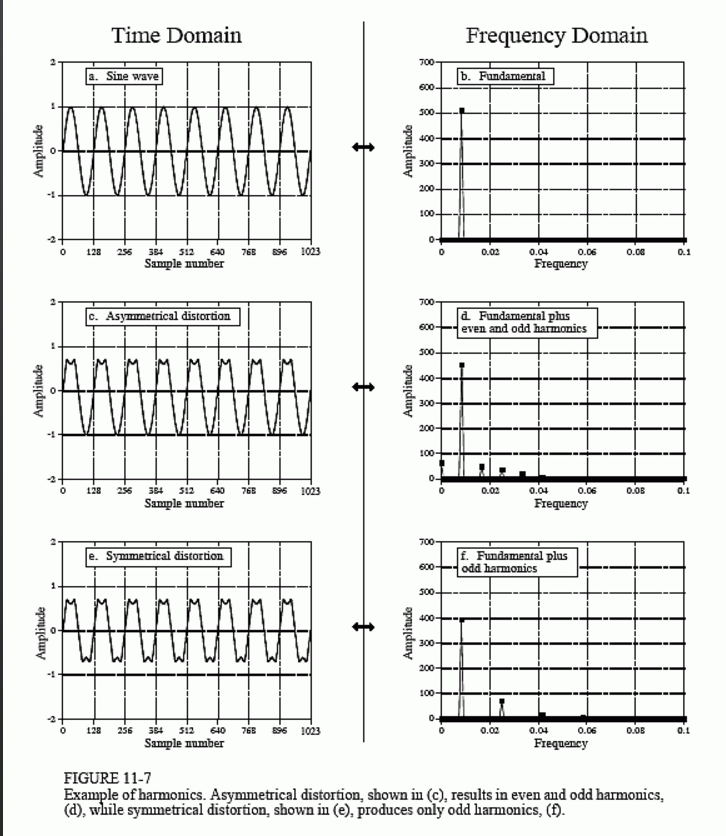
\includegraphics[width=.6\textwidth]{fig1.png}
\caption{\label{fig:fig}Figure 11-7 from "The Scientist and Engineer's Guide to
Digital Signal Processing. Steven W. Smith".}
\end{figure}

\textbf{Figure (e) demonstrates a subtlety of harmonic analysis. If the signal is symmetrical around a horizontal axis, i.e., the top lobes are mirror images of the bottom lobes, all of the even harmonics will have a value of zero.} As shown in (f), the only frequencies contained in the signal are the fundamental, the third harmonic, the fifth harmonic, etc.

All continuous periodic signals can be represented as a summation of harmonics, just as described. Discrete periodic signals have a problem that disrupts this simple relation. As you might have guessed, the problem is aliasing. Figure 11-8a shows a sine wave distorted in the same manner as before, by poking in the tops of the peaks. This waveform looks much less regular and smooth than in the previous example because the sine wave is at a much higher frequency, resulting in fewer samples per cycle. Figure (b) shows the frequency spectrum of this signal. As you would expect, you can identify the fundamental and harmonics. This example shows that harmonics can extend to frequencies greater than 0.5 of the sampling frequency, and will be aliased to frequencies somewhere between 0 and 0.5. You don't notice them in (b) because their amplitudes are too low. Figure (c) shows the frequency spectrum plotted on a logarithmic scale to reveal these low amplitude aliased peaks. At first glance, this spectrum looks like random noise. It isn't; this is a result of the many harmonics overlapping as they are aliased.

\begin{figure}[h]
\centering
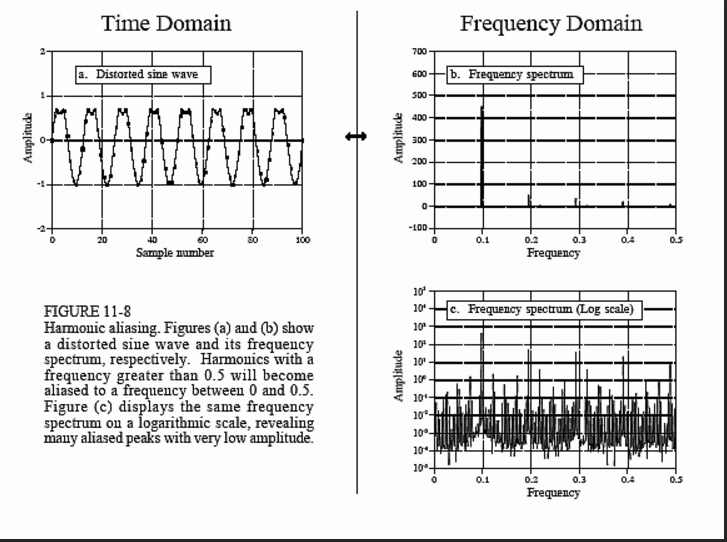
\includegraphics[width=.6\textwidth]{fig2.png}
\caption{\label{fig:fig}Figure 11-8 from "The Scientist and Engineer's Guide to
Digital Signal Processing. Steven W. Smith".}
\end{figure}

It is important to understand that this example involves distorting a signal after it has been digitally represented. If this distortion occurred in an analog signal, you would remove the offending harmonics with an antialias filter before digitization. Harmonic aliasing is only a problem when nonlinear operations are performed directly on a discrete signal. Even then, the amplitude of these aliased harmonics is often low enough that they can be ignored.

The concept of harmonics is also useful for another reason: it explains why the DFT views the time and frequency domains as periodic. In the frequency domain, an N point DFT consists of $\frac{N}{2+1}$ equally spaced frequencies. You can view the frequencies between these samples as (1) having a value of zero, or (2) not existing. Either way they don't contribute to the synthesis of the time domain signal. In other words, a discrete frequency spectrum consists of harmonics, rather than a continuous range of frequencies. This requires the time domain to be periodic with a frequency equal to the lowest sinusoid in the frequency domain, i.e., the fundamental frequency. Neglecting the DC value, the lowest frequency represented in the frequency domain makes one complete cycle every N samples, resulting in the time domain being periodic with a period of N. In other words, if one domain is discrete, the other domain must be periodic, and vice versa. This holds for all four members of the Fourier transform family. Since the DFT views both domains as discrete, it must also view both domains as periodic. The samples in each domain represent harmonics of the periodicity of the opposite domain.





\bibliography{}
\end{enumerate}
\end{document}


